\section{Projektstruktur}\label{sec:projektstruktur}

Ein Electron-Projekt besteht aus zwei Teilen: dem Haupt-/Main-Prozess und dem Rendererprozess.
Der Haupt-/Main-Prozess ist der Prozess, der die \emph{Node.js}-Instanz startet und die \emph{BrowserWindow}-Instanz erstellt, welche den Rendererprozess startet.
Der Rendererprozess ist der Prozess, der die Benutzeroberfläche rendert.
Im Falle des Editors wird die Benutzeroberfläche mit \emph{React} gerendert.

\subsection{Haupt-/Main-Prozess}\label{subsec:haupt-/main-prozess}

\path{src/main/main.ts} ist die Hauptdatei des Haupt-/Main-Prozesses.\\
In der Datei \path{src/main/main.ts} wird die \emph{BrowserWindow}-Instanz erstellt und die \emph{React}-Instanz gestartet.
Des Weiteren werden in der Datei \path{src/main/main.ts} die \emph{IPC}-Nachrichten behandelt, welche vom Rendererprozess gesendet werden.

\subsubsection{IPC}

\emph{IPC} steht für \emph{Inter-Process Communication}.
Im Falle von Electron ist \emph{IPC} ein Mechanismus, der es dem Hauptprozess und dem Rendererprozess ermöglicht, miteinander zu kommunizieren.
\\\\
Der Hauptprozess kann Nachrichten an den Rendererprozess senden, indem die \emph{send}-Methode der \emph{BrowserWindow}-Instanz aufgerufen wird.
Der Rendererprozess kann Nachrichten an den Hauptprozess senden, indem die \emph{send}-Methode der \emph{ipcRenderer}-Instanz aufgerufen wird.
\\\\
Die \emph{IPC}-Nachrichten werden in der Datei \path{src/main/main.ts} behandelt.
Die Handler werden durch die Methode \emph{registerHandlers} alle gemeinsam registriert.

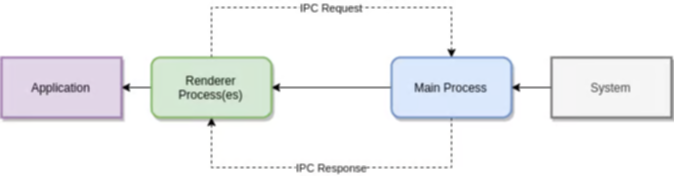
\includegraphics[scale=0.5]{assets/ipcresponserequest}

Hier kann man gut erkennen, wie die \emph{IPC}-Nachrichten zwischen dem Hauptprozess und dem Rendererprozess ausgetauscht werden.
\\\\
Für weitere Informationen zu \emph{IPC} siehe \url{https://electronjs.org/docs/api/ipc-main}.

\subsection{Rendererprozess}\label{subsec:rendererprozess}

\path{src/renderer/index.tsx} ist die Hauptdatei des Rendererprozesses.\\
Der Rendererprozess rendert die Benutzeroberfläche des Editors und verwendet dabei eine \emph{React}-Instanz eines \emph{BrowserWindow}-Objekts.

\subsubsection{React}

Mithilfe von \emph{React} wird die Benutzeroberfläche des Editors gerendert.
Initial wird die \emph{React}-Instanz in der Datei \path{src/renderer/index.tsx} gestartet mit der Methode \emph{run}.
Die \emph{React}-Instanz rendert die Komponente \emph{App} in das \emph{DOM} des \emph{BrowserWindow}-Objekts.
Jedoch, bevor die \emph{React}-Instanz gestartet wird, wird an den Main-Prozess eine \emph{IPC}-Nachricht gesendet (prefetch), um wichtige Daten zu erhalten, wie z.B. die Sprache des Editors, und die Einstellungen des Editors.
Danach wird der Translation-Helper initialisiert und die \emph{React}-Instanz gestartet.

\subsubsection{Translation-Helper}

Der Translation-Helper ist eine Klasse, die die Übersetzungen des Editors verwaltet.
Er wird in der Datei \path{src/renderer/helper/TranslationHelper.ts} implementiert und bildet die Grundlage für die Übersetzungen des Editors.
Er liefert folgende Funktionalitäten:

\begin{itemize}
	\item \emph{translate}: Liefert die Übersetzung für einen bestimmten String in der aktuellen Sprache.
	\item \emph{translateVars}: Liefert die Übersetzung für einen bestimmten String in der aktuellen Sprache und ersetzt dabei Variablen in dem String.
	\item \emph{switchLanguage}: Ändert die aktuelle Sprache des Editors.
	\item \emph{getAvailableLanguages}: Liefert die verfügbaren Sprachen des Editors als ein Array von Enum-Werten.
\end{itemize}

Der Translation-Helper wird in der Datei \path{src/renderer/index.tsx} initialisiert und ist dann global unter \emph{window.t} verfügbar.

\subsubsection{Components}

Der Editor besteht aus 5 Komponenten: \emph{Home}, \emph{BoardConfiguratorV2}, \emph{RiverPresetEditor}, \emph{GameConfigurator} und \emph{Validator}
Diese Komponenten werden in der Datei \path{src/renderer/App.tsx} gerendert.

\paragraph{Home}

\path{src/renderer/screens/Home.tsx} ist die Datei, in der die \emph{Home}-Komponente implementiert ist.\\

Die \emph{Home}-Komponente rendert den Startbildschirm des Editors.
Der Startbildschirm besteht aus 5 Buttons: \emph{Board-Konfigurator}, \emph{Game-Konfigurator}, \emph{Validierer}, \emph{Einstellungen} und \emph{Beenden}.

\paragraph{BoardConfiguratorV2}

\path{src/renderer/screens/BoardConfiguratorV2.tsx} ist die Datei, in der die \emph{BoardConfiguratorV2}-Komponente implementiert ist.\\

Die \emph{BoardConfiguratorV2}-Komponente rendert den \emph{Board-Konfigurator} des Editors.

\paragraph{RiverPresetEditor}

\path{src/renderer/screens/RiverPresetEditor.tsx} ist die Datei, in der die \emph{RiverPresetEditor}-Komponente implementiert ist.\\

Die \emph{RiverPresetEditor}-Komponente rendert den \emph{Fluss-Vorlagen Editor} des Editors.

\paragraph{GameConfigurator}

\path{src/renderer/screens/GameConfigurator.tsx} ist die Datei, in der die \emph{GameConfigurator}-Komponente implementiert ist.\\

Die \emph{GameConfigurator}-Komponente rendert den \emph{Game-Konfigurator} des Editors.

\paragraph{Validator}

\path{src/renderer/screens/Validator.tsx} ist die Datei, in der die \emph{Validator}-Komponente implementiert ist.\\

Die \emph{Validator}-Komponente rendert den \emph{Validierer} des Editors.
